\documentclass[twocolumn,superscriptaddress]{revtex4-1}

\usepackage{hyperref}
\usepackage{verbatim}
\usepackage[font=normalsize]{caption}
\usepackage{mathtools}
\usepackage{relsize}
\usepackage{natbib}

\usepackage{amsmath}
\usepackage{graphicx}
\usepackage[capposition=bottom]{floatrow}
\usepackage{amssymb}
\usepackage{graphicx}
\usepackage{caption}
\usepackage{rotating}
\usepackage{afterpage}
\usepackage{float}
\usepackage{geometry}
\usepackage{titlesec}
\usepackage{epstopdf}

\usepackage{latexsym}
\usepackage{graphicx}
\usepackage{color}
\usepackage{array}
\usepackage{multirow}
\usepackage{wasysym}
\usepackage{verbatim}
\usepackage{subfig}


\addtolength{\oddsidemargin}{-.625in}
\addtolength{\evensidemargin}{-.625in}
\addtolength{\textwidth}{1.25in}
%\addtolength{\voffset}{-70pt}
%\addtolength{\textheight} {120pt}
\newcommand{\isot}[2]{$^{#2}$#1 }
\newcommand{\xeiso}{\isot{Xe}{136}}
\newcommand{\thsrc}{\isot{Th}{228}}
\newcommand{\cosrc}{\isot{Co}{60}}
\newcommand{\krsrc}{\isot{Kr}{83m}}
\newcommand{\cssrc}{\isot{Cs}{137}}
\newcommand{\nonubb}  {$0\nu \beta \beta$}
\newcommand{\gone}{$0.115 \pm 0.003$}
\newcommand{\gtwo}{$5.39 \pm 0.522$}
\newcommand{\fixit}[1]{{\color{red}#1}}

\renewcommand\thesection{\Roman{section}.}
\renewcommand\thesubsection{\arabic{subsection}.}
\renewcommand\thesubsubsection{\alph{subsubsection}.}
\titleformat{\section}[block]{\bfseries\filcenter}{\thesection}{1em}{}
\titleformat{\subsection}[block]{\bfseries\filcenter}{\thesubsection}{1em}{}
\titleformat{\subsubsection}{\bfseries\filcenter}{\thesubsubsection}{1em}{}

\usepackage{titlesec}



%\titleformat{\section}{\bfseries\filcenter}{\thesubsection}{1em}{}
%\titleformat{\subsection}{\bfseries\filcenter}{\thesubsection}{1em}{}
%\titleformat*{\paragraph}{\large\bfseries}
%\titleformat*{\subparagraph}{\large\bfseries}

\begin{document}

\title{Tritium calibration of the LUX detector}

\input{authors}

 \begin{abstract}

We present measurements of the electron-recoil (ER) response of the LUX dark matter detector based upon 170,000 highly pure and spatially uniform fiducial tritium decays. We reconstruct the tritium energy spectrum using the combined energy model and find good agreement with expectations. We report the average charge and light yields of ER events in liquid xenon at 180 V/cm and 105 V/cm and compare the results to the NEST model. We also measure the mean charge recombination fraction as its fluctuations, and we investigate the location and width of the LUX ER band. These results provide input to a re-analysis of the LUX Run3 WIMP search .

\end{abstract}



\maketitle

\section{Introduction}

The LUX collaboration recently reported results from its first underground science run, placing new constraints on WIMP dark matter with masses between 6~GeV and 1~TeV\cite{lux_prl}. LUX is a large dual-phase liquid xenon (LXe) time projection chamber (TPC) with an active mass of ??270?? kg. The primary scintillation light from particle interactions (S1) is collected by two arrays of photomultiplier tubes (PMTs) at the top and bottom of the detector, and the charge signal is converted to light via secondary scintillation at the anode (S2). Measurement of both S1 and S2 allows the event to be located in all three dimensions, and allows discrimination between nuclear recoil (NR) events from electron recoil (ER) events via the ratio (S2/S1).

One of the primary advantages of the liquid TPC technology is its high efficiency for the rejection of external gamma backgrounds via self-shielding. This has enabled the exploration of three orders of magnitude in WMP-nucleon cross-section over the last decade. On the other hand, self-shielding also reduces the effectiveness of external gamma sources such as \cssrc or \thsrc for detector calibration purposes, particularly in the center of the detector and at the low energies relevant for dark matter. In the case of LUX, external gamma source are unable to produce a useful rate of ER calibration events in the fiducial region.  

To address this issue, internal calibration sources that can be dissolved into the liquid xenon and thereby defeat its self-shielding have been developed\cite{Kastens:2009rt}. LUX has deployed two such internal calibration sources; the first based upon \krsrc, and the second based upon tritium ($^{3}$H). \krsrc is a source of two internal conversion electrons at energies of 9.4 keVee and 32.1 keVee separated in time by an intermediate state with a half life of 154 ns. Because it produces two lines in the energy spectrum, \krsrc is well adapted for tracking the spatial and time dependence of the S1 and S2 signals. However, because both \krsrc electrons are above the energy range of interest for dark matter (1.3 - 8 levee), and because the S2 signals from the two electrons generally overlap with each other in the detector,  \krsrc is less useful for constraining the electron recoil (ER) band of the S2/S1 discriminant. 

In this article we describe the development and use of the LUX tritium source, which plays a complementary role to the \krsrc source. Unlike \krsrc, tritium is a single-beta emitter, with a Q value of 18.6 keVee. Its spectral maximum is at 2.5 keVee, and 75\% of its beta decays are below 8 keVee. This allows the detector's ER band to be precisely characterized in a short calibration run without saturating the DAQ. In addition, the tritium spectrum has a finite decay rate extending down to zero keVee, allowing the threshold response of the detector to be studied.

Unlike \krsrc, however, tritium is long-lived, with a half-life of 12.3 years, compared to 1.8 hours for \krsrc. So while the \krsrc is naturally removed from the detector after roughly a day, the tritium must be removed from the liquid xenon by purification. Secondly, tritium must be introduced into the detector in a manner which will not impair the charge or light collection properties of the detector. This is less of a concern with \krsrc, because it can be passed through the LUX getter prior to entering the detector owing to its noble nature. 

Tritiated methane (CH$_3$T) was chosen as the appropriate host molecule to deliver the activity into LUX. Methane has several desirable chemical and physical properties compared to T$_2$: first, its diffusion constant (D) times solubility (K) is ten times smaller in common LUX materials such as teflon (PTFE) and polyethylene (PE)\cite{miyake:1983}, mitigating the problem of back-diffusion of activity into the liquid xenon after purification; it is chemically inert, so it is not expected to adhere to surfaces (as the T$_2$ molecule is known to do), and it is consistent with good charge transport in liquid xenon.

Our goal was to develop a (CH$_3$T) source which could be safely injected into LUX and removed such that any residual activity that remained (due to back-diffusion from plastics or inefficient purification) should be no more than 0.33 $\mu$Bq, which is 5\% of the LUX ER background rate design goal for a 30,000 kg$\cdot$days exposure. We desired to collect a LUX calibration dataset of $\sim$15,000 tritium events, roughly a factor of 100 larger than the number of expected ER background events in LUX. 


\section{Injection and removal of CH$_3$T}

Two CH$_3$T sources with total activities of 3 Bq and 200 Bq were prepared for use in LUX. Each source is contained in a 2.25 liter stainless steel bottle and is mixed with 2 atmospheres of LUX-quality purified xenon. The xenon acts as a carrier gas to extract the source from the bottle. The CH$_3$T was synthesized by Moravek Biochemical~\cite{moravek} and delivered at a specific activity of 0.1 milliCurie per millimol.

The injection system is shown in Fig.~\ref{fig:plumbing}. A fraction of the source bottle activity may be extracted by allowing the carrier gas to expand into one or more expansion volumes consisting of various sections of evacuated tubing. The amount of extracted activity is controlled by selecting an expansion volume of appropriate size. A methane purifier (SAES model MC1-905F\cite{seas}) located between the source bottle and the expansion volume ensures that only CH$_3$T, CH$_4$, and noble gases are allowed to enter the system. The extracted activity is then injected into the TPC by diverting a small portion of the LUX xenon gas flow through the expansion volumes. 

\begin{figure}[h!]
\includegraphics[width=80mm]{fig/TritiumPlumbing.png}
\caption{Plumbing diagram of the CH$_3$T injection system for LUX. CH$_3$T is injected downstream of the xenon gas purifier so that it passes through the detector prior to being removed.  Red arrows indicate the direction of flow.}
\label{fig:plumbing}
\end{figure}

The CH$_3$T appears in the TPC within minutes of the injection, and is removed via the normal action of the LUX xenon purification system, which operates without interruption during the entire procedure. Its centerpiece is a hot zirconium getter (SAES model PS4-MT15-R1\cite{seas}) that acts upon gaseous xenon and continuously removes all non-noble species including methane. The xenon gas flow is driven by a diaphragm pump at a rate of $\sim$27 standard liters per minute (slpm). 

Prior to the first injection of CH$_3$T activity, we first confirmed that the LUX getter unit was capable of efficient methane removal by injecting  $\sim$1 ppm (part-per-million g/g) of natural methane (CH$_4$) into LUX. As shown in Appendix~\ref{sec:appendix1}, the CH$_4$ concentration in the gas, monitored with a mass spectrometer, was observed  to decrease exponentially with a time constant of 5.9 $\pm 0.07$ hours. The one-pass efficiency of the getter for CH$_4$ removal was measured to be 97\% under the LUX flow and temperature conditions by sampling the gas before and after the getter. 

On August 8, 2013, an initial injection of 20 mBq of CH$_3$T was performed, followed five days later by an injection of 800 mBq. The count rate of fiducial single-scatter events with S1 $<$ 150 photons detected (phd) (roughly the endpoint of the tritium beta spectrum) is shown in Fig.~\ref{fig:ch3t_removal}. The CH$_3$T activity is clearly observed, with the count rate reaching its maximal value in one hour. For both injections the activity was removed with a six-hour exponential time constant similar to that observed in the CH$_4$ injection. It is worth noting that the observed purification time constant is considerably shorter than the xenon mass turn-over time of LUX (about 40 hours for 370 kg of xenon).  The origin of the short purification time remains under investigation. The location of the CH$_3$T events from the first injection after all corrections is shown in Fig.~\ref{fig:event_location}. As expected, the events are uniform within the detector volume.� An empirical model that describes the removal of CH$_3$T from LUX is presented in Appendix~\ref{sec:appendix2}.

\begin{figure}[h!]
\includegraphics[width=90mm]{fig/CH3T_Rate.eps}
\caption{Rate of single scatter events with S1 below 150 phd in the fiducial volume during the August 2013 CH$_3$T injections.  The solid lines are exponential fits to the activity vs. time.}
\label{fig:ch3t_removal}
\end{figure}


 
\begin{figure}[h!]
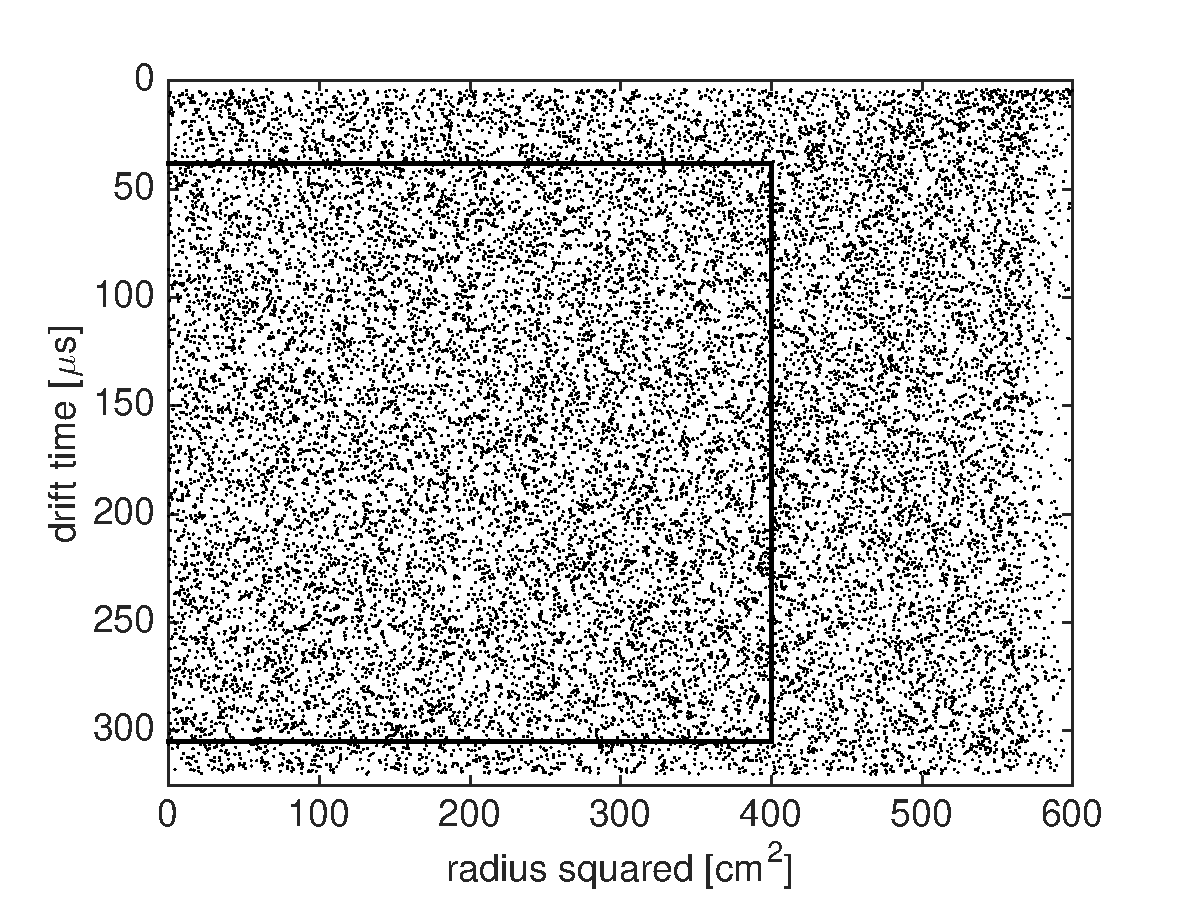
\includegraphics[width=90mm]{fig/rz_scatter.eps}
\caption{The location of events in drift time vs. detector radius squared for the August 2013 CH$_3$T injection. The drift time is a proxy for the $z$ coordinate of the event. The solid black line represents the fiducial volume used in Ref.~\cite{lux-reanalysis}.}
\label{fig:event_location}
\end{figure}







\input{results}

\section{Summary}

We have characterized the electron recoil response of the LUX dark matter experiment with a tritium calibration source. The large dataset, high event purity, and the simple nature of the decay provide a powerful tool to study the detector and to investigate the fundamental properties of LXe as a particle detection medium for WIMP searches. 

We find strong evidence in support of the combined energy model for ER events in the WIMP energy range, and we report new measurements of the light and charge yields, the average recombination, and the fluctuations in the recombination as a function of energy. We have determined that the width of the ER band in LUX is driven by fluctuations in the number of detected S1 photons. We find a small number of outlier events far below the ER band centroid out of 170,000 fiducial tritium decays, consistent with background expectations in this dataset.

The results presented here are used in an improved analysis of the Run 3 WIMP search data to determine the location and width of the LUX ER band and to measure the fiducial volume~\cite{lux-reanalysis}. Additional tritium data has also been collected in support of the on-going LUX Run4 WIMP search and is presently under analysis.

\appendix

\subsection{Outgassing of Tritiated Methane from Plastics}
\label{sec:appendix}

\newcommand*{\Scale}[2][4]{\scalebox{#1}{$#2$}}%

An accurate model of a tritiated methane injection into LUX must account for outgassing of CH$_3$T from plastics such as polyethylene and teflon. Duhamel's priciple, an integral solution to Fick's second law on a half-infinite line is found to be
\[\Scale[0.85]{\phi (x,t) = KC_{out} - \int \limits_0^t erf(\frac{x}{\sqrt{4D(t - \tau)}})K\dot{C_{out}}(\tau)d\tau - KC_{out}(0)erf(\frac{x}{\sqrt{4Dt}}),}\]
where $K$ is the solubility of the material, $D$ is the diffusion constant, and $C_{out}$ is the concentration at the surface of the material. 
%\cite{Piche}
For the outgassing process we are only able to detect the flux of material out of the plastic.  This is given by Fick's first law evaluated at $x=0$,
\[J_{out}(t)= - K \sqrt{\frac{D}{\pi}}\left( \int \limits_0^t \frac{\dot{C_{out}}(\tau)}{\sqrt{t-\tau}} d \tau + \frac{C_{out}(0)}{\sqrt{t}}\right),\]
where the sign has been flipped since the flux of material is outward.  It is no longer possible to evaluate $K$ and $D$ separately, since the diffusion in and out of the plastic is completely determined by the time-dependent concentration outside of the plastic.  To simplify our model, we define a new constant
\[ G = K \sqrt{ \frac{D}{ \pi }} .\] Using data from the LUX sampling system we set an upper limit of $G<0.0016 \frac{cm}{\sqrt{day}}$. 

\begin{figure}[h!]\centering
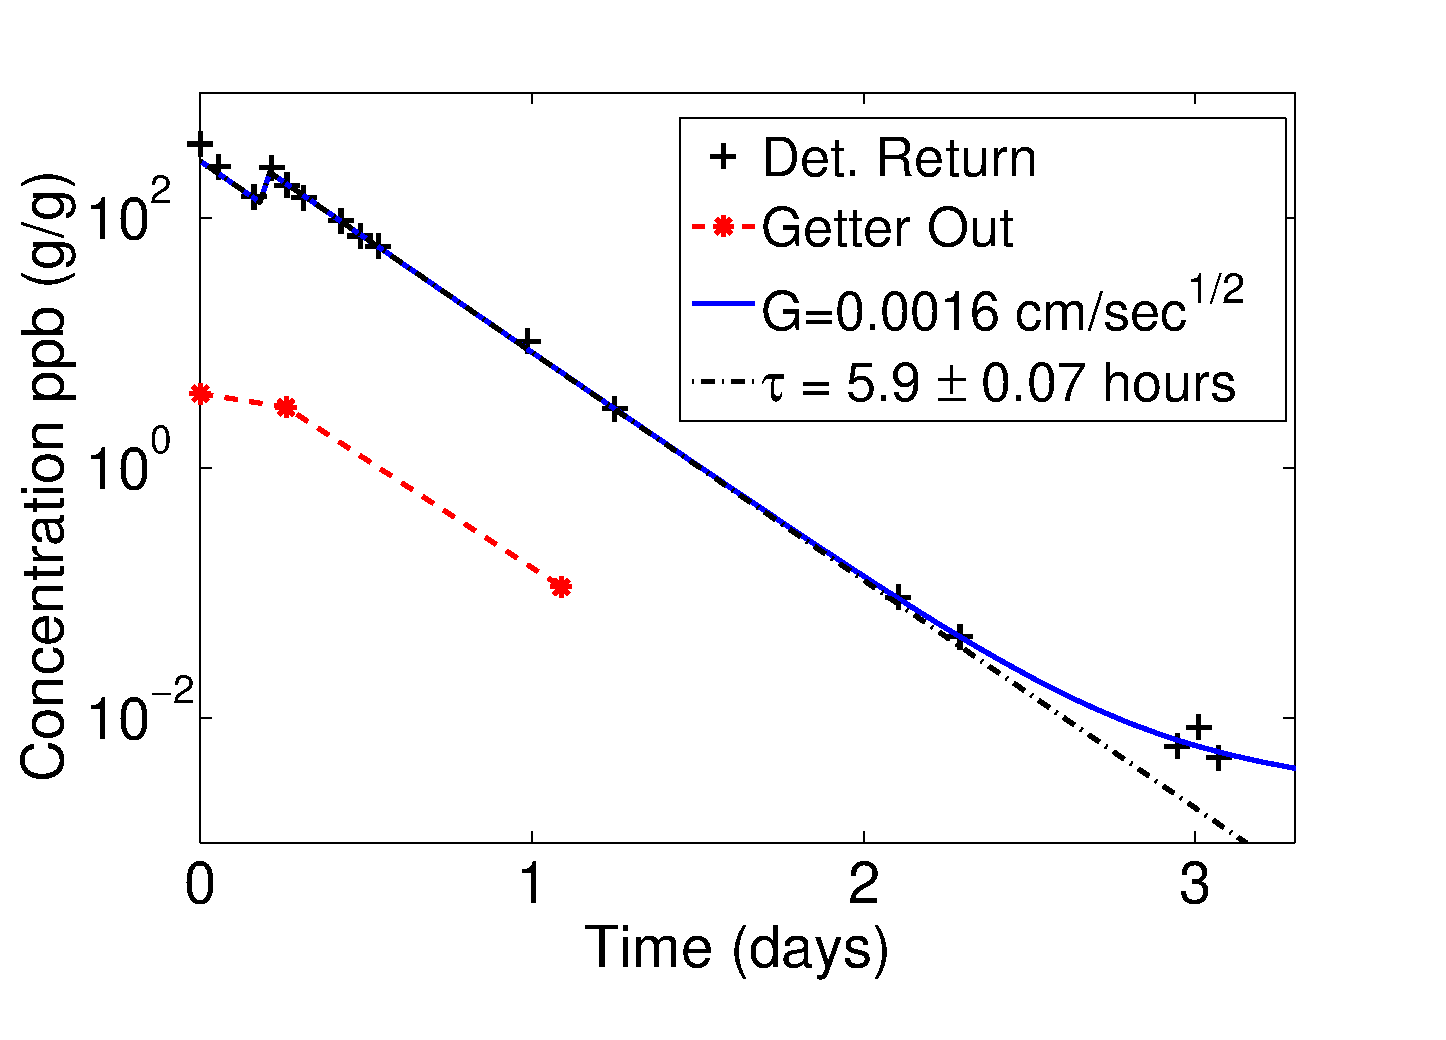
\includegraphics[width=80mm]{fig/July_CH4_wOG.eps}
\caption{Removal of natural methane observed by the integrated xenon sampling system prior to the tritiated methane injections. The red points indicate measurements at the getter outlet, we find a 97\% one pass removal efficiency at a flow rate of 27 SLPM. The blue curve shows the upper limit on the effect of outgassing from the plastics. The black dashed lines shows the exponential fit to the natural methane removal from the xenon with a time constant of 5.9 $\pm 0.07$ hours. $\rm 5\times10^{-3}$ ppb (g/g) is the limit of detection for methane.}
\label{fig:ch4_removal}
\end{figure}

With a constraint on $G$ taken from the analytic solution to Fick's second law, we turn to numerical simulation to answer the question of how much initial CH$_3$T activity to inject into LUX to meet our calibration goals. We set a limit of 0.33 $\mu$Bq (5\% of the LUX ER background rate design goal) from residual CH$_3$T activity after an injection.  Several assumptions are made to simplify the numerical model.  First, we approximate the diffusion into plastic as being a one dimensional process.  Since the plastic in LUX can be approximated by a cylindrical shell there is no dependence on the azimuthal or $z$ coordinates.  Since $r$ is large compared to the thickness of the plastic shell, $\frac{\delta^2 \phi}{\delta r^2} \gg \frac{1}{r} \frac {\delta \phi}{\delta r}$, so Fick's laws in a one dimensional approximation become
\[J=-D\frac{\delta \phi}{\delta r}\vec{r}\]
\[\frac{\delta \phi}{\delta t} = D \frac{\delta^2 \phi}{\delta r^2}.\]  We assume the concentration of CH$_3$T in LUX is uniform throughout its volume, since the design of LUX creates currents which stir the liquid xenon.  With perfect mixing the effect of the purifier can be modeled by adding an exponential time dependence of 5.9 $\pm 0.07$ hours to the outer volume. 

We use a simple implementation of the first order Euler method for to produce numerical simulations of the residual activity in LUX after a CH$_3$T injection. The diffusion is simulated by setting the concentration at the boundary of the piece equal to $KC_{out}$, where $C_{out}$ is the concentration of CH$_3$T in the xenon.  This concentration is dependent on time according to
\[\frac{\delta C_{out}}{\delta t} = J_{out} \frac{A_{plastic}}{V_{xenon}}-\frac{C_{out}}{\tau},\]
where $A_{plastic}$ is the surface area of the plastic cylinder, $V_{xenon}$ is the total volume of xenon in the fiducial region, and $\tau$ is the characteristic removal time of methane from LUX.  The first term on the right of this equation models outgassing of CH$_3$T from the plastic cylinder, while the second term models removal of CH$_3$T through purification.  Using the first order Euler method, we arrive at an expression for $C_{out}$ given by
\[C_{j+1}=C_j + \Delta t \left[(J_{1,j}-J_{N_x,j})\frac{A_{plastic}}{V_{xenon}}-\frac{C_j}{\tau}\right].\]
The initial concentration is defined by dividing the desired injection activity by the volume of the fiducial region.  We choose $D = 2.3 \times 10^{-9} \frac {cm^2}{sec}$ so that the half-infinite boundary conditions in our diffusion model is valid, and combine this with our upper limit on $G$ to extract a value for $K$.  We use this model to predict the total number of calibration events as well as the time required to return to \textless 5\% of the nominal background rate for any CH$_3$T injection into LUX.  

\begin{figure}[h!]
\centering
\includegraphics[width=0.95\textwidth]{fig/LUX_og_lim.eps}
\caption{Displayed are the results of simulated outgassing effects from a 1 Bq (black curve) and 10 Bq (red curve) injections of CH$_3$T into LUX. The dashed blue line is the tritium activity goal of 0.33 $\mu$ Bq. The simulated outgassing assumes the upper limit of G taken from the CH$_4$ injection in LUX (0.0016 cm/day$^{1/2}$).}
\label{fig:tau_var}
\end{figure}

Figure \ref{fig:tau_var} shows the results of our simulations for a 1 Bq and 10 Bq injection into LUX.  We find that for moderate injections on the order of 1 Bq we reach our limit of 0.33 $\mu$Bq 8 days after the initial injection.  For larger injections it can take longer than 35 days to reach our background limit.  While these simulations use a conservative upper limit for the value of $G$ it emphasizes that injecting too much CH$_3$T into LUX can lead significant delays in a WIMP search.  


\subsection{Tritiated Methane Removal}
\label{sec:RD}

The removal efficiency of zirconium getters for CH4 in xenon had previously been studied at the University of Maryland.  It was found that greater than 99.99\% of natural methane can be removed in a single pass through a zirconium getter. \cite{Dobi_CH4} Tritiated methane is chemically identical to natural methane, so it follows that similar removal efficiencies should be expected for CH$_3$T.  To verify this a small scale tritiated methane injection system was integrated into a liquid xenon system at the University of Maryland.  This system used a SAES MC1-905F methane purifier placed in series immediately after the CH$_3$T source bottle to prevent non-methane species of tritium from entering the plumbing. Over 68,000 Bq of observed CH$_3$T activity was injected into this small scale system and a removal efficiency of over 99.99\% for tritiated methane in xenon was confirmed.

\begin{figure}[h!]\centering
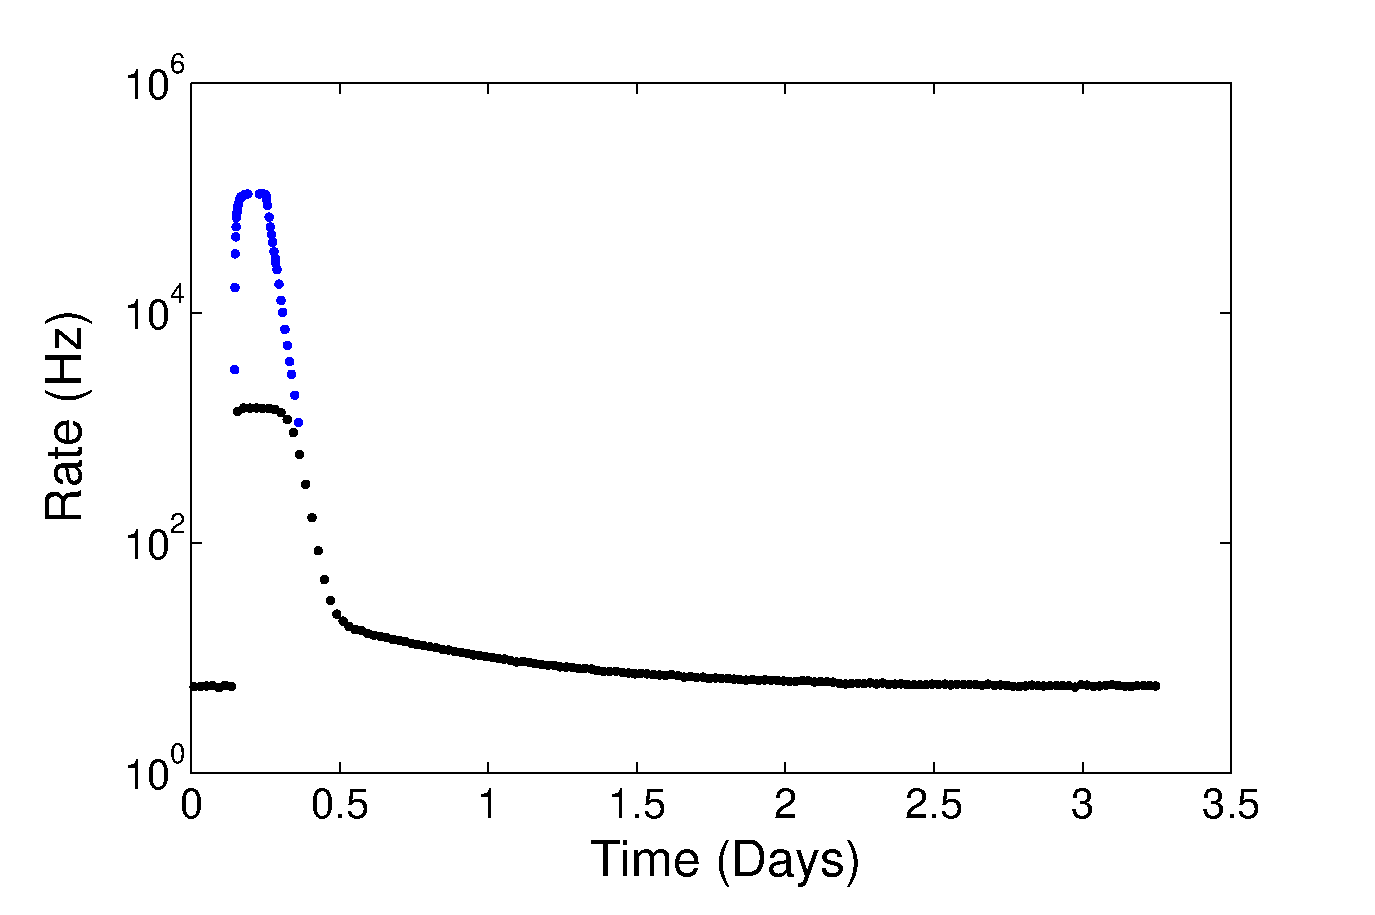
\includegraphics[width=80mm]{fig/TimeHisto_Analog2.eps}
\caption{A time histogram of the event rate during a tritium injection into our small scale detector. The event rate greatly exceeded the limits of our ADC (black data points), so a analog scalar was used to count the true event rate (blue data points). }
\label{fig:Density}
\end{figure}



%\begin{acknowledgments}

%\end{acknowledgments}

\bibliographystyle{thesisbibstyle}
\bibliography{Tritium}


\end{document}